\section{単純モデルでの解析}
単純モデルでの解析は、Code\_Aster 10で記述されたCAELinuxの投稿をCode\_Aster 14で実施しました。
\vspace{-\baselineskip}
\subsection{ジオメトリ}
5(mm)×12(mm)×43(mm)のブロック形状を使用
\begin{itemize}
	\item 上下の2つのエリア:AtopとAbot
	\item 2節点グループ
	      \begin{itemize}
		      \item 底面の中心節点:Nfixx
		      \item y軸の最端位置にある2つの節点:Nfixy
	      \end{itemize}
\end{itemize}
\vspace{-\baselineskip}
\begin{figure}[htbp]
	\caption{ブロック上に定義された4つのグループ}
	%\label{fig:}
	\centering
	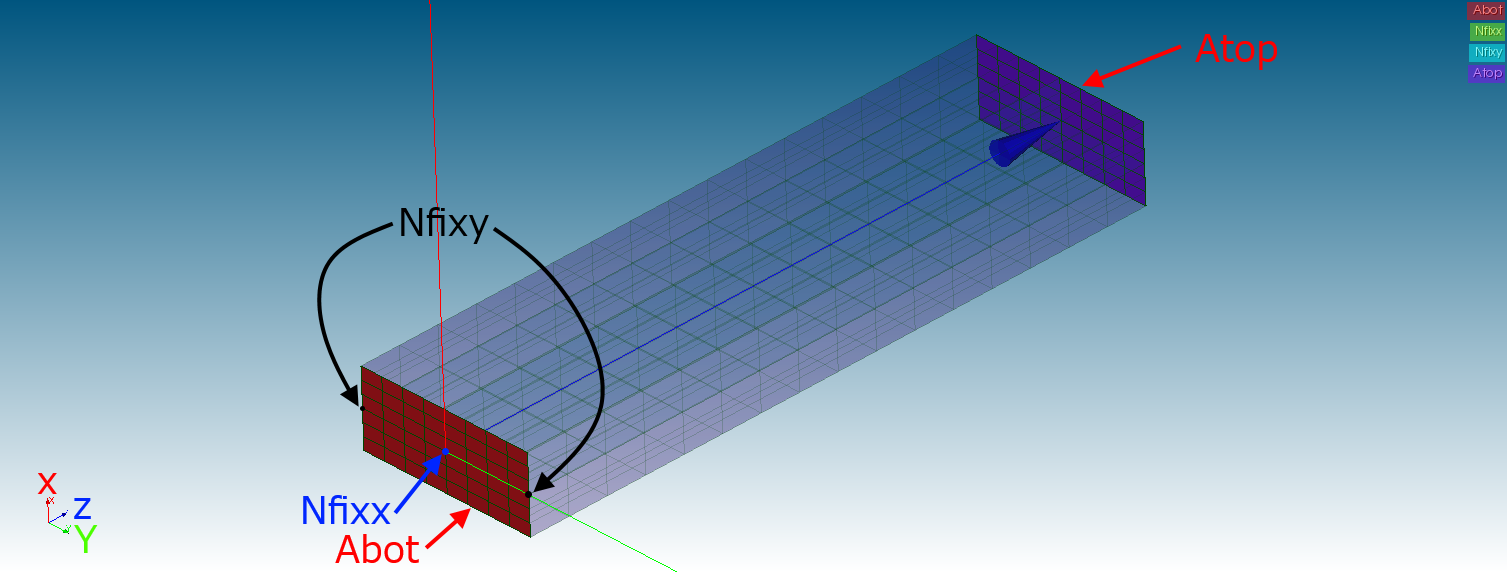
\includegraphics[width=0.7\columnwidth]{fig/bc.png}
\end{figure}
\clearpage
\subsection{コマンド}
材料特性は、Mooney-Rivlin(ムーニー・リブリン)型の材料モデルで設定しています。
\begin{lstlisting}[caption =材料設定, label=材料設定]
mater = DEFI_MATERIAU(ELAS_HYPER=_F(C01=2.3456,
                                    C10=0.709,
                                    C20=0.0,
                                    NU=0.499))
\end{lstlisting}
\begin{lstlisting}[caption =拘束条件, label=拘束条件]
mecabc = AFFE_CHAR_MECA(DDL_IMPO=(_F(DZ=0.0,
                                     GROUP_MA=('Abot', )),
                                  _F(DY=0.0,
                                     GROUP_NO=('Nfixx', )),
                                  _F(DX=0.0,
                                     GROUP_NO=('Nfixy', ))),
                        MODELE=model)
\end{lstlisting}
\begin{lstlisting}[caption =荷重条件, label=荷重条件]
mecach = AFFE_CHAR_MECA(MODELE=model,
                        PRES_REP=_F(GROUP_MA=('Atop', ),
                                    PRES=-6.0))
\end{lstlisting}
\clearpage
\begin{lstlisting}[caption =非線形解析コマンド, label=非線形解析コマンド]
resnonl = STAT_NON_LINE(CHAM_MATER=fieldmat,
                        COMPORTEMENT=_F(DEFORMATION='GROT_GDEP',
                                        RELATION='ELAS_HYPER'),
                        CONVERGENCE=_F(ITER_GLOB_MAXI=20),
                        EXCIT=(_F(CHARGE=mecabc),
                               _F(CHARGE=mecach,
                                  FONC_MULT=func)),
                        INCREMENT=_F(LIST_INST=listr),
                        MODELE=model,
                        NEWTON=_F(REAC_ITER=1))
\end{lstlisting}
\clearpage
\subsection{結果}
\subsubsection{変位}
上のエリアAtopに-6(MPa)の圧力荷重を20等分してかけています。\\
次の左図は、この荷重の全体的な変位を示しています。\\表示されている変位は、実際の変位です(デフォルメ表示はしていません)。\\
最終的なZ方向変位は34.4(mm)で、ひずみは34.4÷43=0.8($\epsilon$)です。\\
右図は圧力-12(MPa)のときのZ方向変位を示しています。\\
上面の最大変位は182.5(mm) で、ひずみは182.5÷43=4.2($\epsilon$)です。
\begin{figure}[H]
	\begin{minipage}{0.48\hsize}
		\caption{圧力荷重-6(MPa)の場合}
		%\label{}
		\centering
		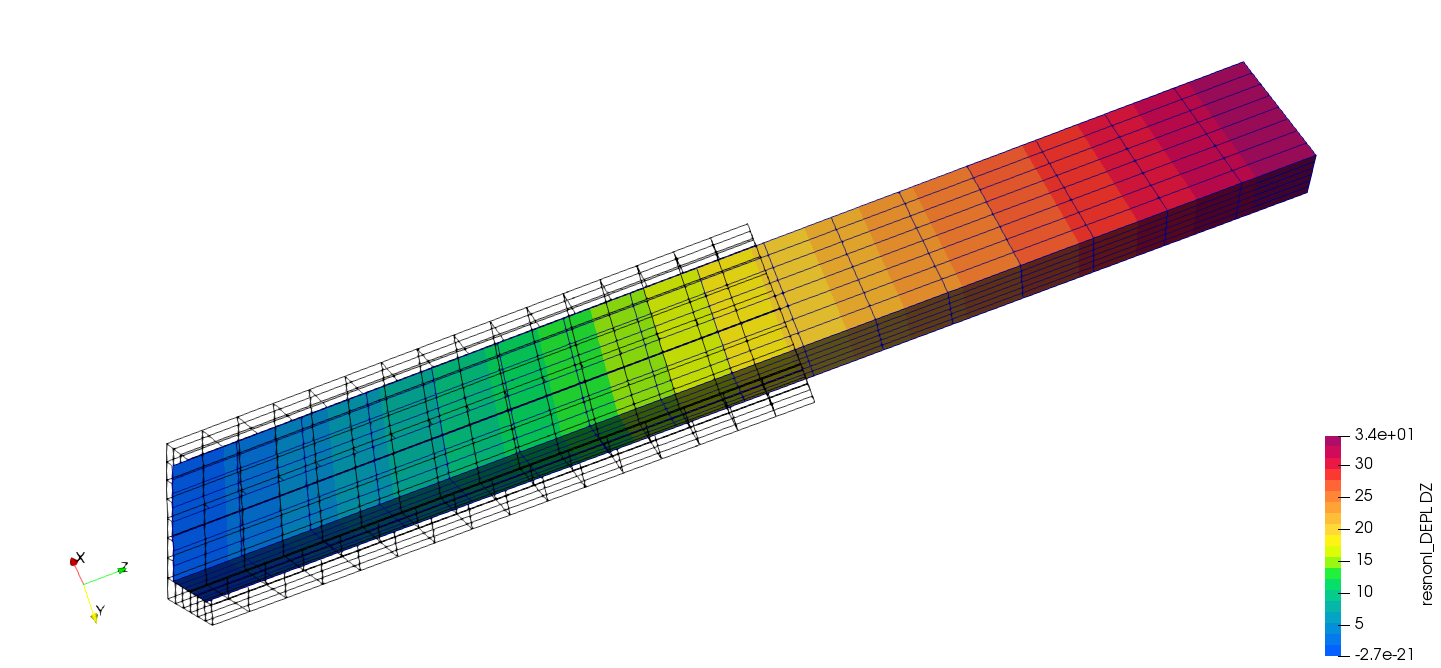
\includegraphics[width=0.9\columnwidth]{fig/6MPa.png}
	\end{minipage}
	\begin{minipage}{0.48\hsize}
		\caption{圧力荷重-12(MPa)の場合}
		%\label{}
		\centering
		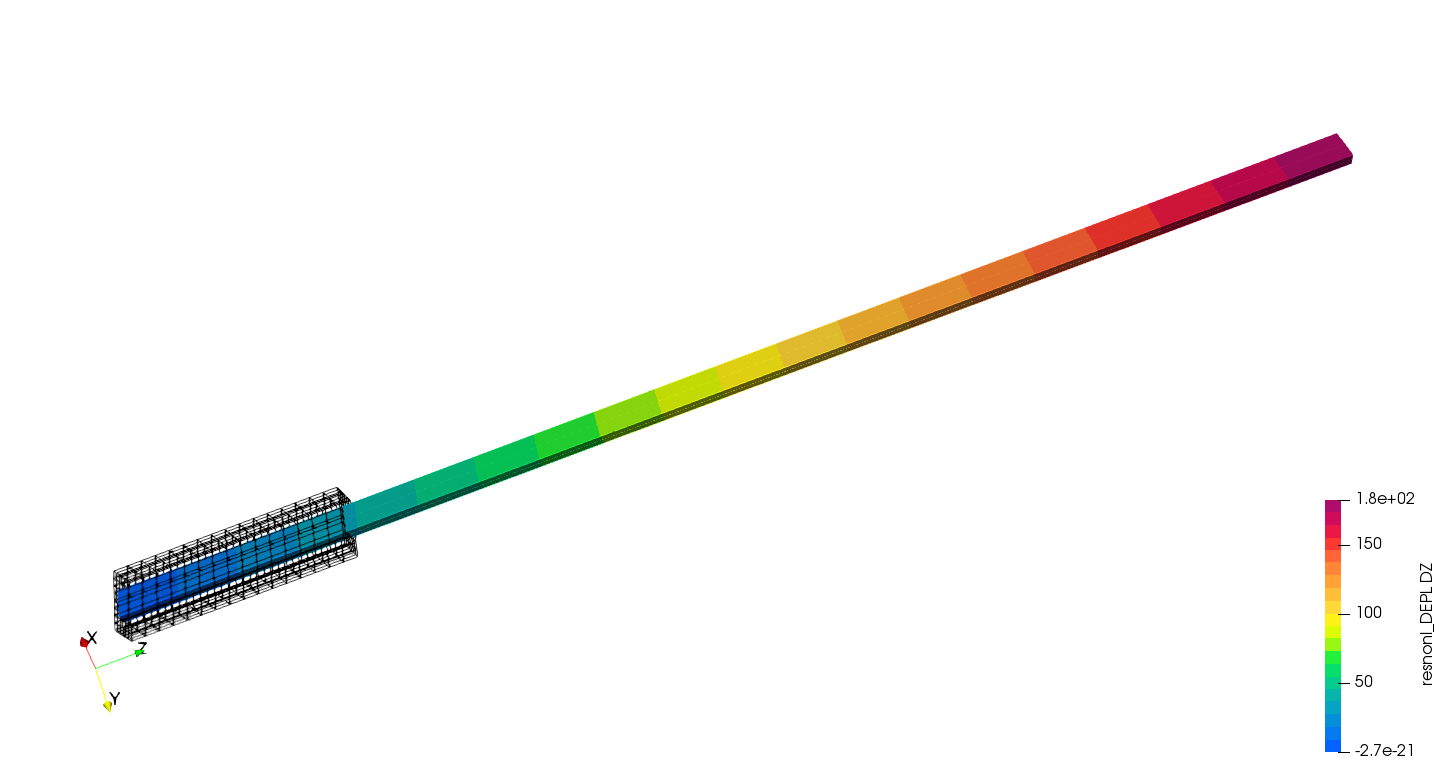
\includegraphics[width=0.9\columnwidth]{fig/12MPa.png}
	\end{minipage}
\end{figure}
\clearpage
\subsubsection{体積変化}
ここでは、-6(MPa)の圧力荷重の場合について説明します。\\
次の図は、X、Y、Z方向の変位量を示しています。\\
各方向の最大変位量は次のとおりです。
\begin{figure}[H]
	\begin{minipage}{0.32\hsize}
		\caption{X方向変位量:0.64(mm)\\(両方向)}
		%\label{}
		\centering
		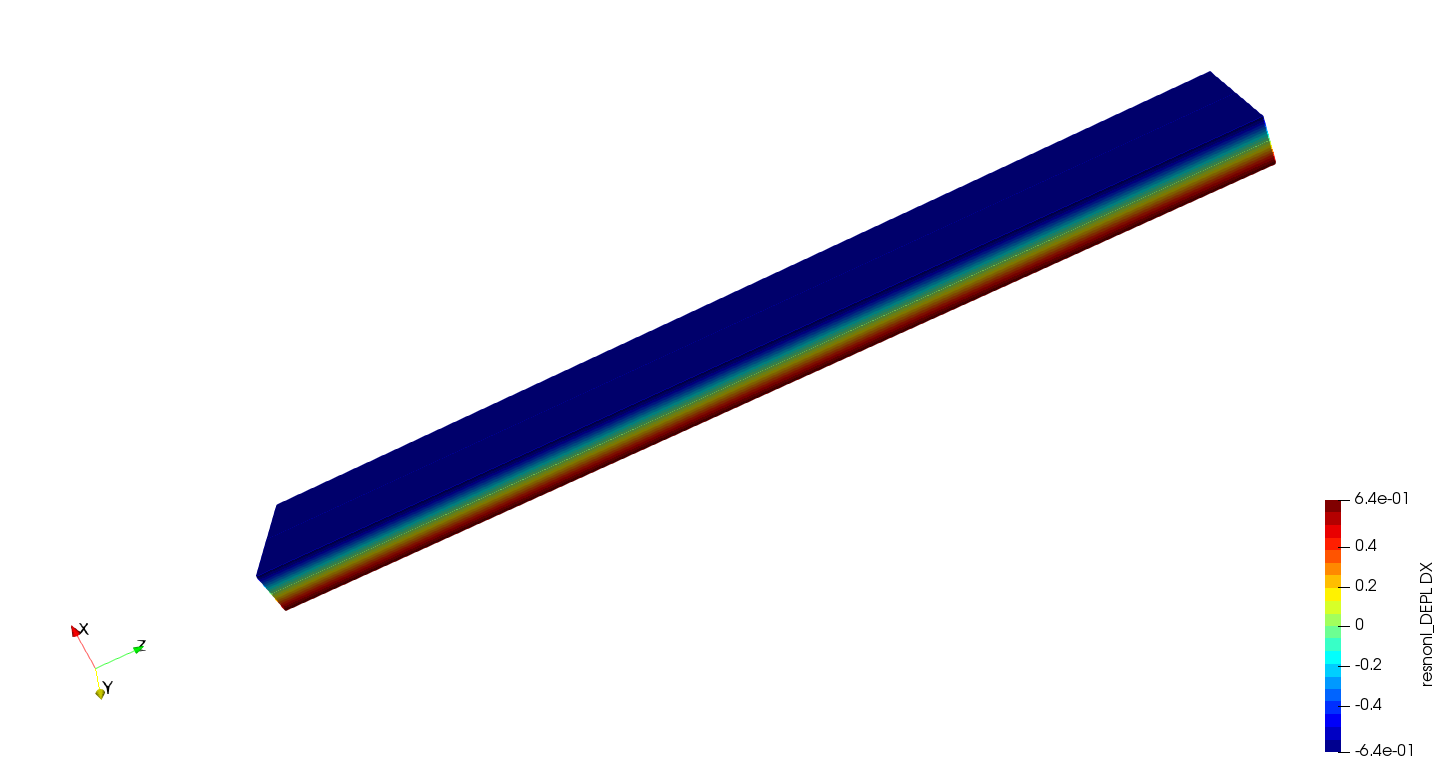
\includegraphics[width=0.9\columnwidth]{fig/dispX.png}
	\end{minipage}
	\begin{minipage}{0.32\hsize}
		\caption{Y方向変位量:1.5(mm)\\(両方向)}
		%\label{}
		\centering
		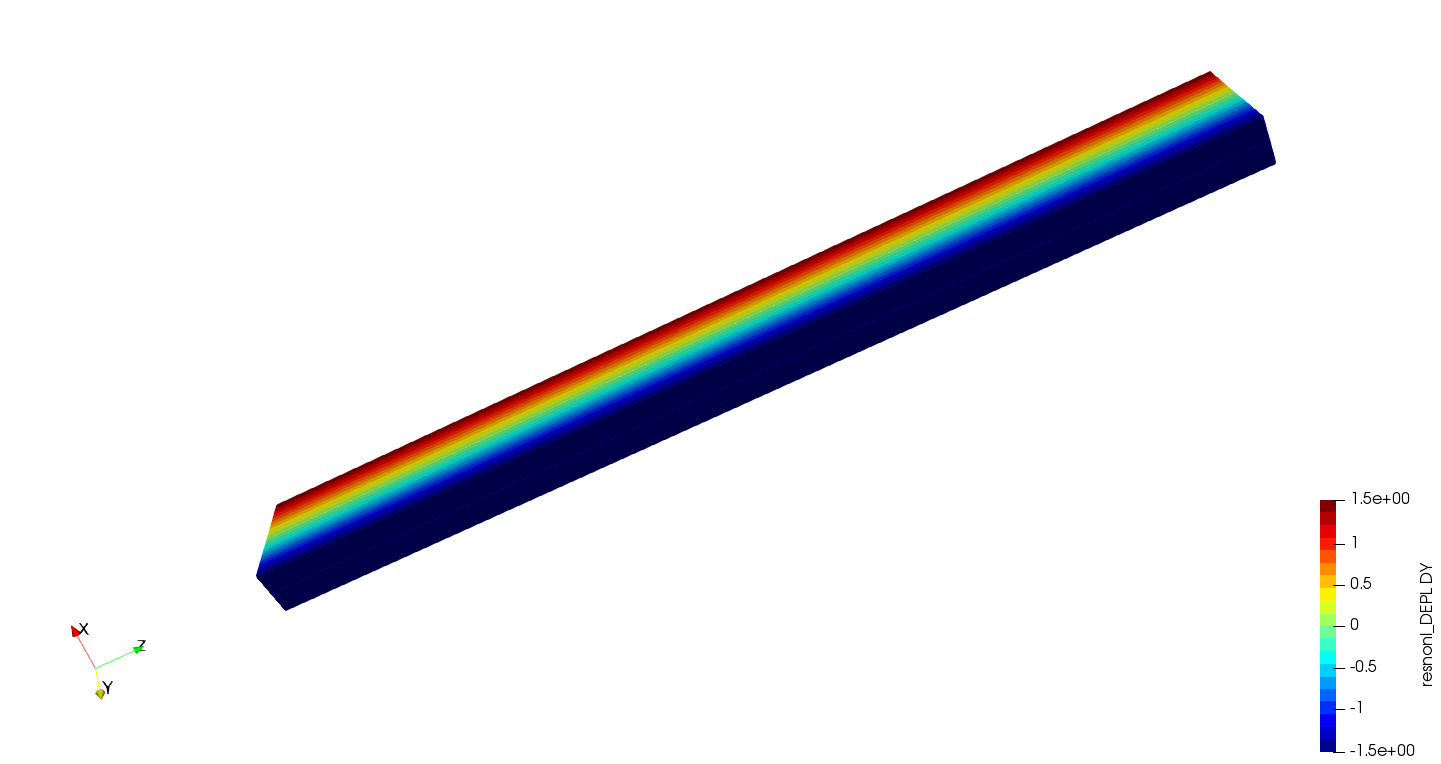
\includegraphics[width=0.9\columnwidth]{fig/dispY.png}
	\end{minipage}
	\begin{minipage}{0.32\hsize}
		\caption{Z方向変位量:34.4(mm)\\(正方向のみ)}
		%\label{}
		\centering
		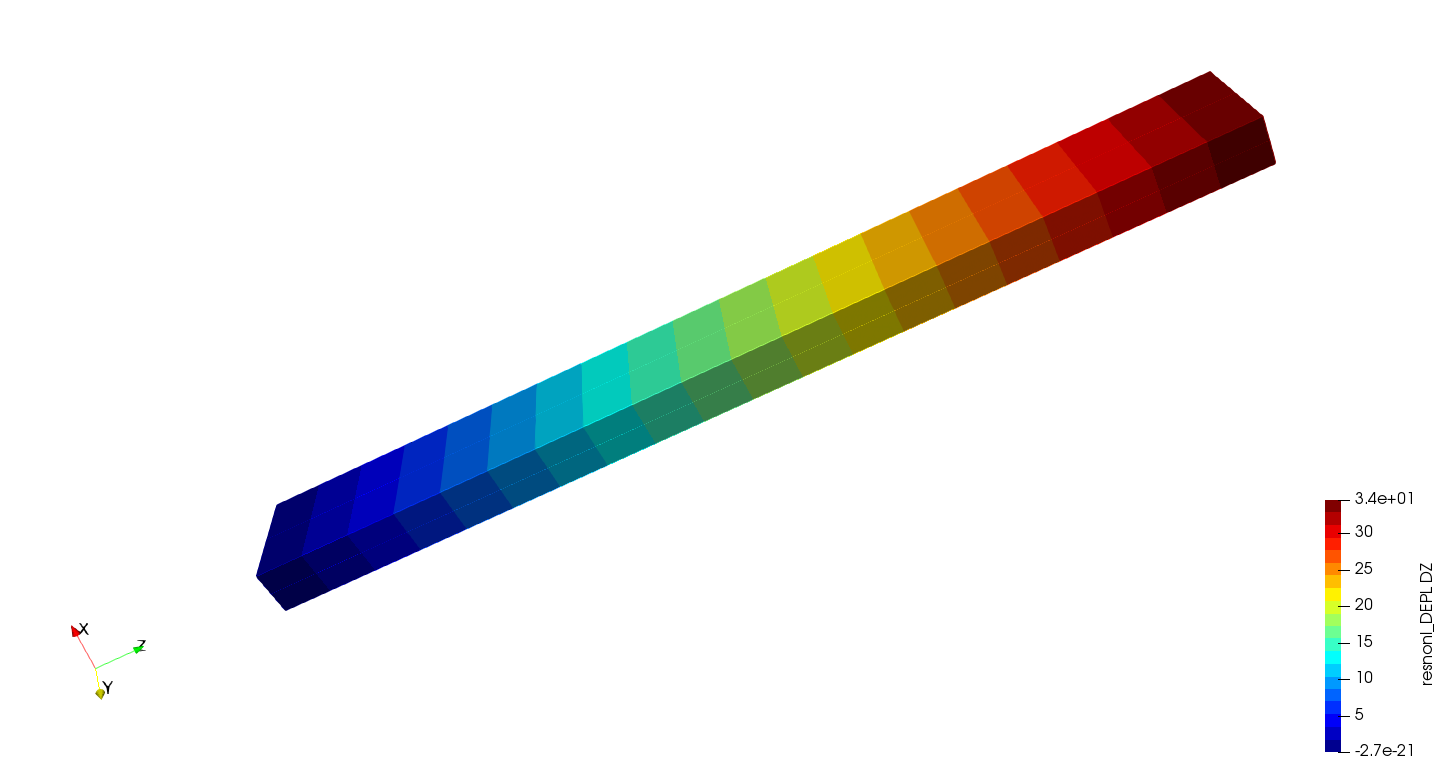
\includegraphics[width=0.9\columnwidth]{fig/dispZ.png}
	\end{minipage}
\end{figure}
ポアソン比$\nu$は、0.499にしたので、体積はほとんど変わらないと予想され、\\
変形前の体積は:
\begin{equation}
	% \label{}
	V_{0}=5\times12\times43=2,580(mm^{3})
\end{equation}
変形後の体積は:
\begin{equation}
	% \label{}
	V_{def}=2(2.5-0.64)\times2(6-1.5)\times(43+34.4)=2,591(mm^{3})
\end{equation}
体積変化は:11($mm^{3}$)でした。